\documentclass[11pt]{beamer}
\usepackage[utf8]{inputenc}
\usepackage[T1]{fontenc}
\usepackage{lmodern}
\usetheme{default}
\usepackage{mathptmx}
\usepackage{graphicx}
\usepackage[style=apa, backend=biber,natbib=true]{biblatex}
\addbibresource{References.bib}
\usepackage{geometry}
\begin{document}
	\title{Quantifying the Status of Galamsey In Ghana With Time Series Classification}
	\author{Kalong Boniface\\ Fugah Seletey Mitchell}
	%\subtitle{}
	%\logo[scale=0.01]{
\includegraphics{H:/Boni Project/Latex/Proposal/uenrlogo.png}}
	\institute{University Of Energy and Natural Resource, Sunyani\\
		Department of Mathematics and Statistics}
	%\date{}
	%\subject{}
	%\setbeamercovered{transparent}
	%\setbeamertemplate{navigation symbols}{}
	\begin{frame}[plain]
		\maketitle
	\end{frame}
	
	\begin{frame}
		\frametitle{Introduction}
	The purpose of this paper is to establish an understanding of time series analysis on remotely sensed data. Which will introduced us to the fundamentals of time series modeling, including decomposition, autocorrelation and modeling historical changes in Galamsey Operation in Ghana, the Cause,Dangers and it's Environmental Impact.\\
Galamsey("gather them and sell")\parencite{OwusuNimo2018}, is the term given by local Ghanaian for illegal small-scale gold mining in Ghana\parencite{DavidYawDanquah2019}
	\end{frame}
    \begin{frame}
    	\begin{block}{Problem Statement}
             	The Footprint of Galamsey is Spreading at a much faster rate.
    	\end{block}
    \end{frame}
    \begin{frame}
    	\frametitle{Overview}
    	
    The purpose  is to establish an understanding in time series analysis on remotely sensed data. We will be introduced to the fundamentals of time series modeling, including decomposition, autocorrelation and modeling historical changes.\\
         \begin{itemize}
		\item  Perform time series analysis on satellite derived vegetation indices\\
		\item  Gain familiarity with R Markdown, Reticulate and the R Spatial Ecosystem\\
		\item  Process satellite imagery using the Google Earth Engine API\\
		\item  Create a Statistical  interactive dashboard\
         \end{itemize}
    \end{frame}
    \begin{frame}
    	\frametitle{Data collection and Methodology}
    	%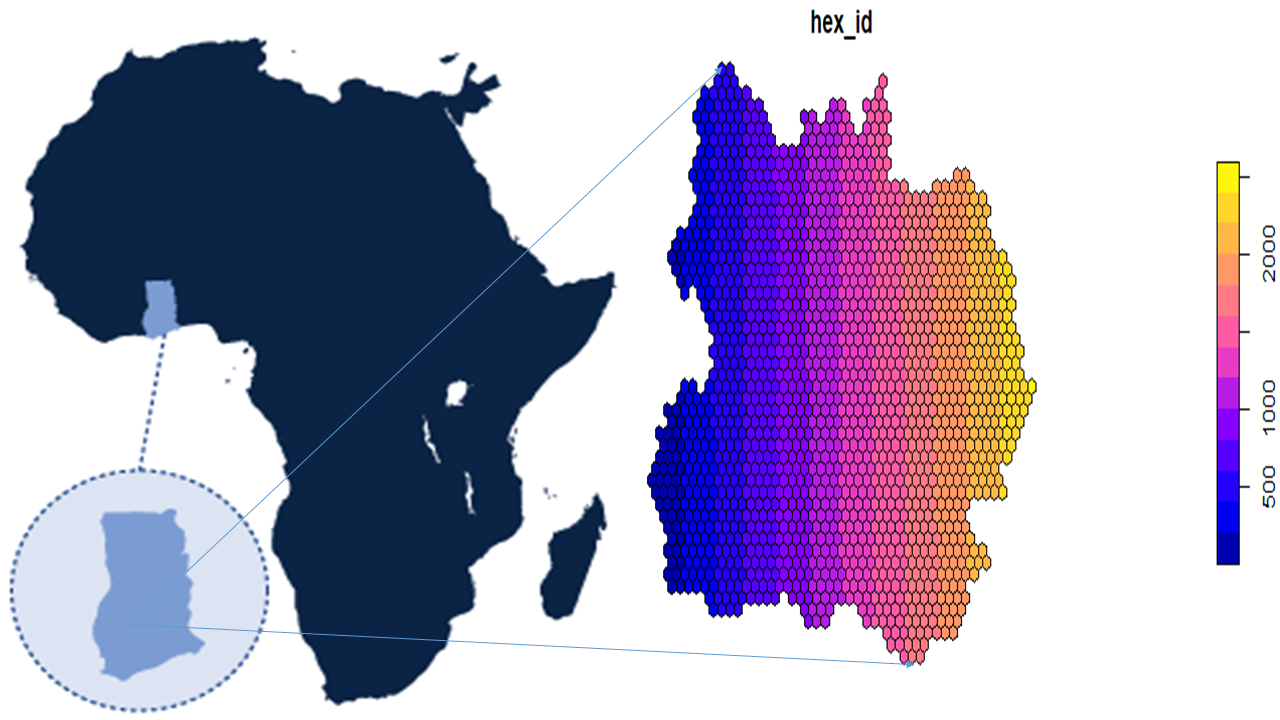
\includegraphics[scale=0.2]{H:/Boni Project/Latex/Proposal/Presentation1.png}
    \end{frame}
     \begin{frame}
     	\frametitle{}
     	\begin{itemize}
     \item	First, we will pull Sentinel 2 to select NDVI and EVI data from Google Earth Engine, applying a quality filter to mask poor quality pixels.\\	
     \item	Instead of performing our analysis on the imagery itself, we will be summarizing the mean NDVI and EVI value , this will allow the analysis to take less time while producing a visually appealing and informative map.\\	
     \item	Some cells may not contain NDVI and EVI for a given month, to correct this, we will apply  smoothing method using an ARIMA function.\\	
    \item 	Once NA values are remove, we will decompose the time series to remove seasonality and fit a linear model to the normalized data.\\	
    \item 	Once we have extracted the linear trend, we will then make a move to classifier our data on the map and map it.
     \end{itemize}
     \end{frame}
 \begin{frame}
 \begin{block}{Limitations}
  The aims to build an explanatory model of the data without over fitting the problem set, to use as simple a model as possible while accounting for as much of the data as possible. When breaking down time series data into component parts, remote sensing data has additional limitations that make this more challenging. It is almost inevitable that you will not get this same level of precision from remote sensing data. Additionally, atmospheric conditions can skew the visual results, where the hue of the vegetation changes drastically from image to image due to atmospheric conditions such as (fog, ground moisture, cloud cover).
 \end{block}
\end{frame}
\begin{frame}
	\frametitle{References}
	\printbibliography[]
\end{frame}
\end{document}